\section{Diagramme de séquence}
Nous représentons le scénario de la déviation d'une route vers un trou noir en utilisant le diagramme de séquence.
\newline
L'utilisateur de l'application web dans cet exemple est l'administrateur réseaux. On suppose que l'administrateur réseaux veut dévier une route par son adresse IP source. 
\newline
Lorsque l'opération est terminée, donc l'application web confirme que c'est fait, la route est ensuite serait stockée dans la base de données afin que le client puisse aller consulter les routes qui ont été déviées.
\\
\\
\begin{figure}[h]
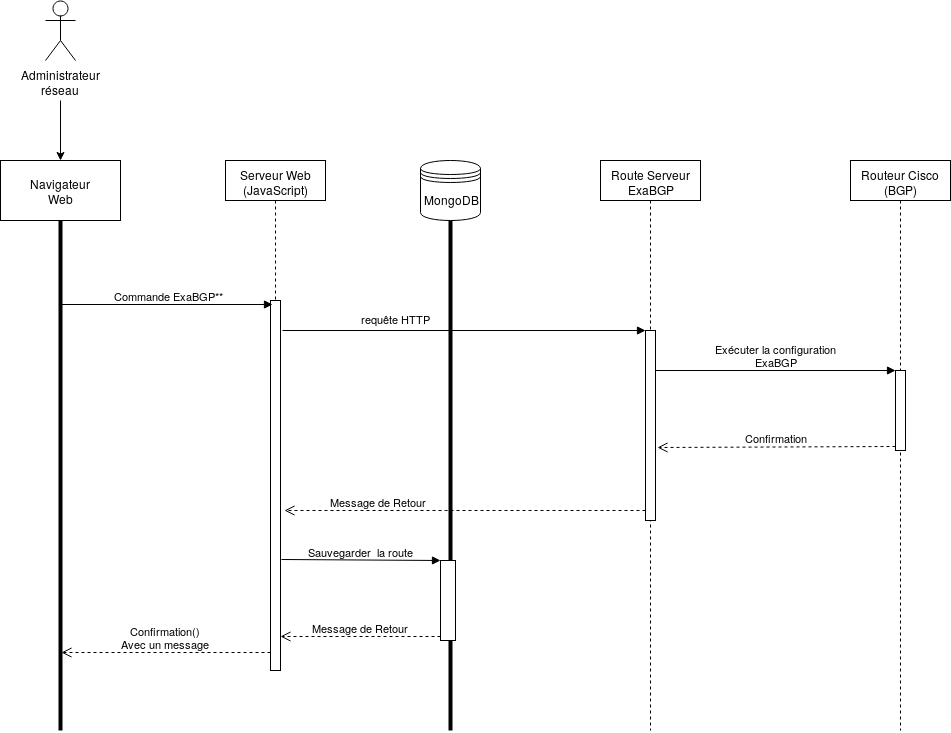
\includegraphics[scale = 0.5]{img/diagramme_de_sequence.png}
Commandes ExaBGP:
\begin{itemize}
\item show neighbor [optional neighbor ip] summary
\item show neighbor [optional neighbor ip] extensive
\item show neighbor [optional neighbor ip] configuration
\item show ajd-rib in [extensive] 
\item show ajd-rib out [extensive] 
\item announce watchdog
\item announce route 
\item announce eor
\item announce flow
\item announce operational
\item announce vpls
\item announce route-refresh
\end{itemize}
\end{figure}


\begin{figure}[h]
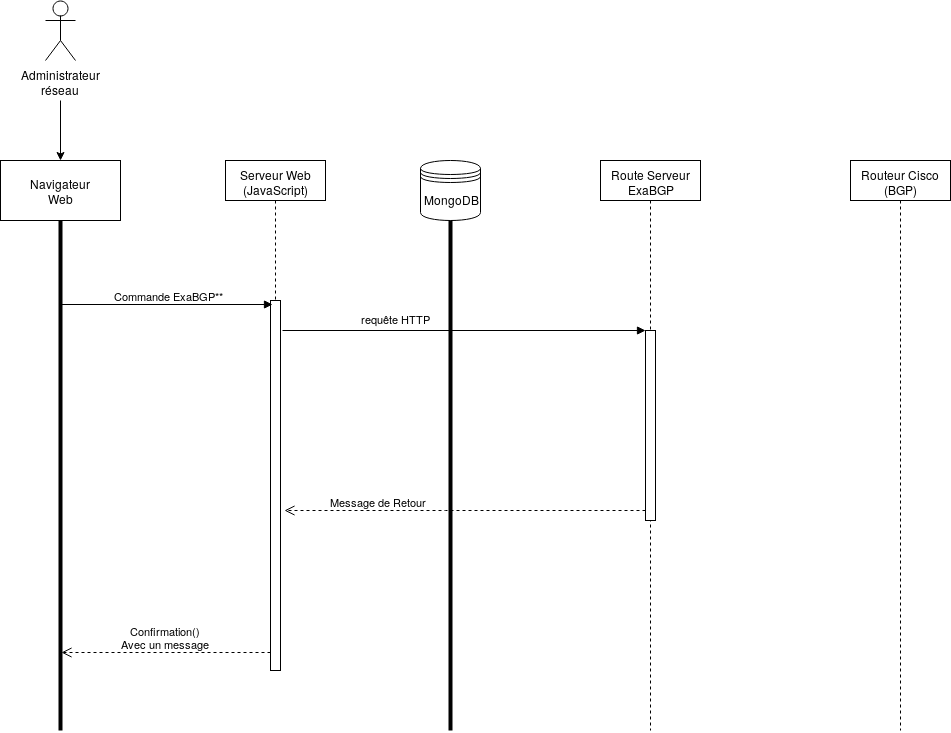
\includegraphics[scale = 0.5]{img/diagramme_de_sequence2.png}
Commandes ExaBGP:
\begin{itemize}
\item shutdown
\item reload 
\item restart 
\item version
\item teardown
\end{itemize}
\end{figure}


\begin{figure}[h]
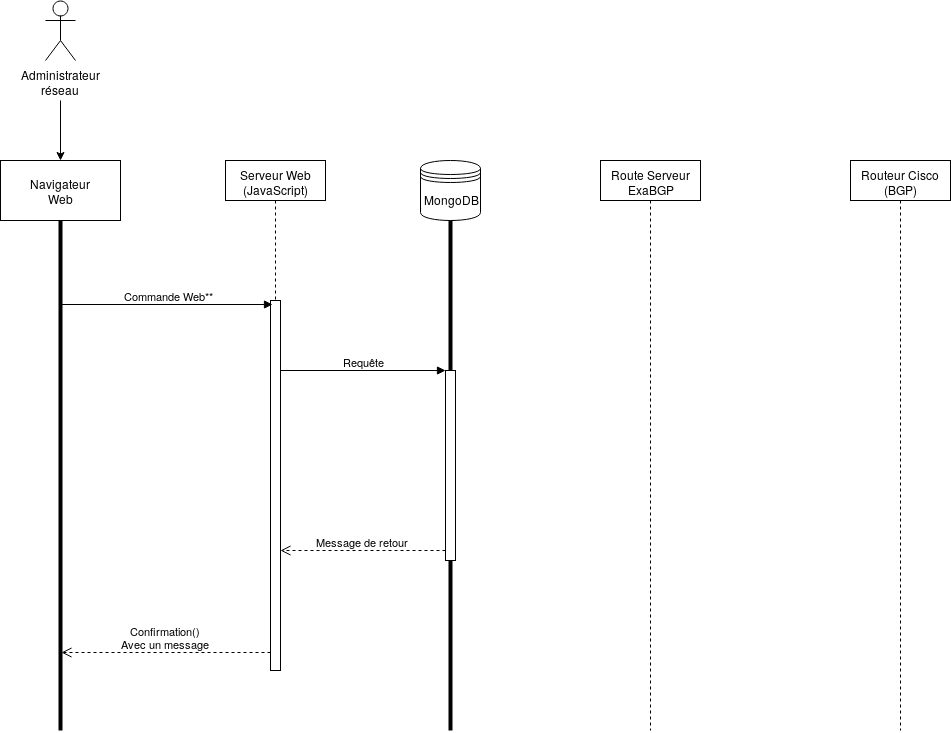
\includegraphics[scale = 0.5]{img/diagramme_de_sequence3.png}
Commandes Web:
\begin{itemize}
\item Recherche route
\item Connections
\end{itemize}
\end{figure}

